\begin{frame}
    \frametitle{Getting help from the FEniCS community}
    \begin{center}
        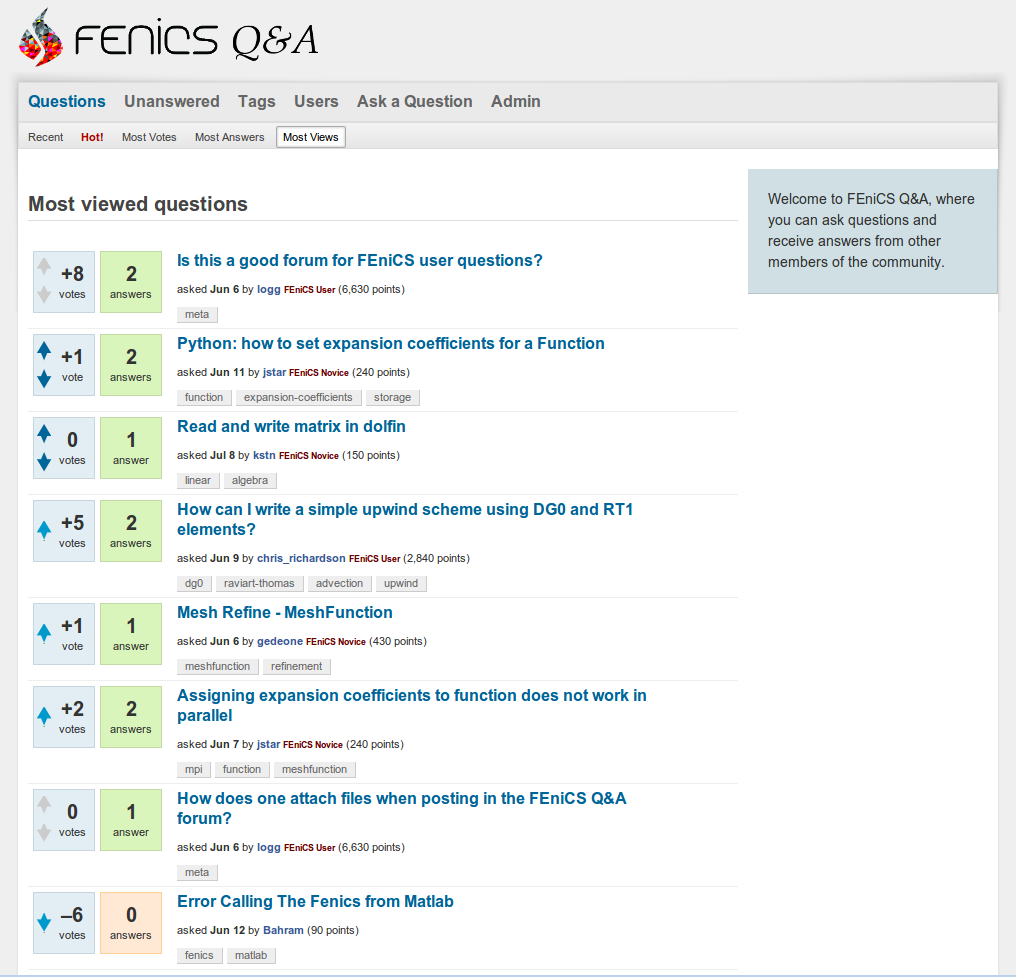
\includegraphics[height=0.75\textheight]{png/qa_overview.png}
        \vspace{1em}
        \small
        \colemph{\url{http://fenicsproject.org/qa/}}
    \end{center}
\end{frame}

\begin{frame}
    \frametitle{Getting help from the FEniCS community}
    \begin{center}
        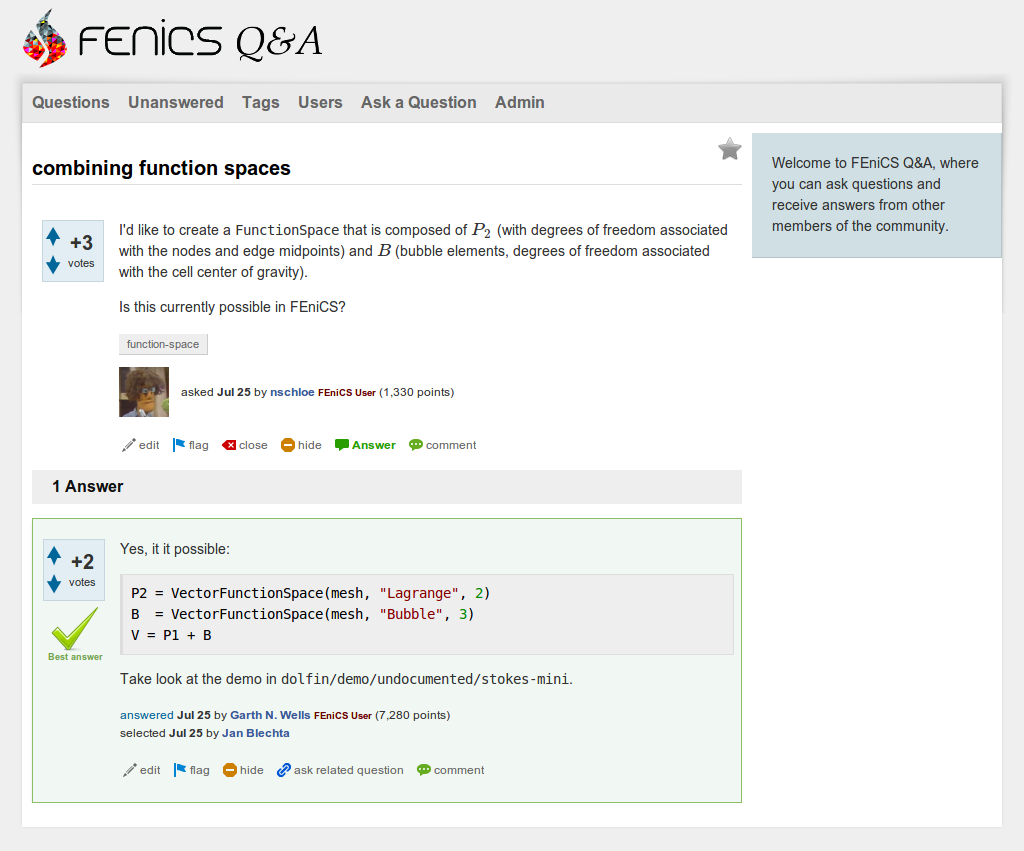
\includegraphics[height=0.75\textheight]{png/qa_example.png}
        \vspace{1em}
        \small
        \colemph{\url{http://fenicsproject.org/qa/}}
    \end{center}
\end{frame}

\begin{frame}
  \frametitle{Community resources}

  \linespread{1.5}
  \begin{itemize}
  \item
    The FEniCS mailing list

    \url{fenics@fenicsproject.org}
  \item
    The FEniCS QA forum

    \url{http://fenicsproject.org/qa/}
  \item
    The FEniCS Google+ community

    \url{http://plus.google.com/}
  \item
    Twitter

    \url{\#fenicsproject}
  \item
    The FEniCS developer site (Bitbucket)

    \url{https://bitbucket.org/fenics-project/}
  \end{itemize}
  \linespread{1.0}

  \vspace{0.1cm}

  \begin{center}
    \underline{\colemph{\url{http://fenicsproject.org/}}}
  \end{center}

\end{frame}
